\documentclass{beamer}
\usetheme{Warsaw}
\usepackage[utf8x]{inputenc}
\usepackage[german]{babel}
\usepackage{color}
\usepackage{xcolor}
\usepackage{listings}
\usepackage{caption}
\DeclareCaptionFont{white}{\color{white}}
\DeclareCaptionFormat{listing}{\colorbox{gray}{\parbox{\textwidth}{#1#2#3}}}
\captionsetup[lstlisting]{format=listing,labelfont=white,textfont=white}
\lstset{
 language=Java,
 basicstyle=\footnotesize\ttfamily, % Standardschrift
 numbers=left,               % Ort der Zeilennummern
 numberstyle=\tiny,          % Stil der Zeilennummern
 stepnumber=5,              % Abstand zwischen den Zeilennummern
 numbersep=5pt,              % Abstand der Nummern zum Text
 tabsize=2,                  % Groesse von Tabs
 extendedchars=true,         %
 breaklines=true,            % Zeilen werden Umgebrochen
 frame=b,         
 %commentstyle=\itshape\color{LightLime}, Was isch das? O_o
 %keywordstyle=\bfseries\color{DarkPurple}, und das O_o
 basicstyle=\small,
 stringstyle=\color[RGB]{42,0,255}\ttfamily, % Farbe der String
 keywordstyle=\color[RGB]{127,0,85}\ttfamily, % Farbe der Keywords
 commentstyle=\color[RGB]{63,127,95}\ttfamily, % Farbe des Kommentars
 showspaces=false,           % Leerzeichen anzeigen ?
 showtabs=false,             % Tabs anzeigen ?
 xleftmargin=17pt,
 framexleftmargin=17pt,
 framexrightmargin=5pt,
 framexbottommargin=4pt,
 showstringspaces=false      % Leerzeichen in Strings anzeigen ?        
}
\newcommand\Fontvi{\fontsize{6}{7.2}\selectfont}
\begin{document}
\title{FHNW APSI Lab 2 : Html Form}   
\author{Roland Hediger, Jonas Schwammberger} 

\date{\today} 

\frame{\titlepage} 

\begin{frame}
\section*{Übersicht}
\tableofcontents
\end{frame} 

\begin{frame}
 \section{Einleitung}
 \begin{itemize}
  \item Java HTTP Servlet Applikation
  \item MVC Pattern - kein Framework 
  \item 1 Servletklasse 
  \item mehrere Methoden die auf 1 Controller aufrufe machen.
  \item 1 Model - Company.java - DAO mithilfe JDBC
 \end{itemize}
\end{frame}

\begin{frame}
 \section{Robuste Programmierung im Controller und Model}
 \begin{itemize}
 \item Information Hiding - soviel private und final wie möglich
 \item Controller zustandslos behalten. Hat nur die Verantwortung für DB Verbindung
 \item Nach Setzen von Properties im DAO werden die Werte automatisch zuerst als nicht gültig betrachtet.
  \item Annotationen begrentzt eingesetzt
 \end{itemize}
\end{frame}
\begin{frame}[fragile]
 \section*{Validierung von Inputs}
 \begin{itemize}
  \item Globale Valid Variable
  \item \texttt{List<String> messages} wird gefüllt mit Benachrichtigungen beim Auftreten von Fehler.
  \item Nur falls valid = true ist im Company kann ein Eintrag gespeichert werden.
  \item Jeder Formulareintrag wird gegen ein ``CleanString'' (Regexausdruck) gematcht.
  \item Passwort Wechsel :
  \item Seperate Validerung , eingeben von altes Passwort vorrausgesetzt .
 \end{itemize}
\begin{figure}[h]
 \centering
 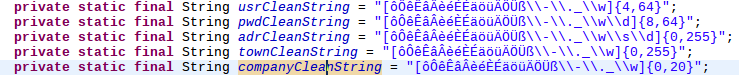
\includegraphics[scale=0.4]{./code.png}
 % code.png: 739x82 pixel, 72dpi, 26.07x2.89 cm, bb=0 0 739 82
\end{figure}


\end{frame}

\begin{frame}[fragile]

\section{Views}
Einsatz von JSP:\\
\begin{lstlisting}
   request.setAttribute("messages", messages);
			request.getRequestDispatcher(REGISTER).forward(request, response);
\end{lstlisting}
\end{frame}
  
\begin{frame}[fragile]
Beispiel JSP Seite :
\begin{lstlisting}[language=html]
  <form method="POST" action='/apsi_lab2/RattleBits' name="login">
  <ul class="error">
<%
    List<String> messages = (List<String>)request.getAttribute("messages");
	Iterator<String> it = messages.iterator();
    while (it.hasNext()) {
%>
	<li><%= it.next() %></li>
<% } %>
</ul>

\end{lstlisting}
\end{frame}



\begin{frame}
\section*{Ende}
 \huge Danke für Ihre Aufmerksamkeit.
\end{frame}

\end{document}

